% Options for packages loaded elsewhere
\PassOptionsToPackage{unicode}{hyperref}
\PassOptionsToPackage{hyphens}{url}
%
\documentclass[
]{book}
\usepackage{amsmath,amssymb}
\usepackage{iftex}
\ifPDFTeX
  \usepackage[T1]{fontenc}
  \usepackage[utf8]{inputenc}
  \usepackage{textcomp} % provide euro and other symbols
\else % if luatex or xetex
  \usepackage{unicode-math} % this also loads fontspec
  \defaultfontfeatures{Scale=MatchLowercase}
  \defaultfontfeatures[\rmfamily]{Ligatures=TeX,Scale=1}
\fi
\usepackage{lmodern}
\ifPDFTeX\else
  % xetex/luatex font selection
\fi
% Use upquote if available, for straight quotes in verbatim environments
\IfFileExists{upquote.sty}{\usepackage{upquote}}{}
\IfFileExists{microtype.sty}{% use microtype if available
  \usepackage[]{microtype}
  \UseMicrotypeSet[protrusion]{basicmath} % disable protrusion for tt fonts
}{}
\makeatletter
\@ifundefined{KOMAClassName}{% if non-KOMA class
  \IfFileExists{parskip.sty}{%
    \usepackage{parskip}
  }{% else
    \setlength{\parindent}{0pt}
    \setlength{\parskip}{6pt plus 2pt minus 1pt}}
}{% if KOMA class
  \KOMAoptions{parskip=half}}
\makeatother
\usepackage{xcolor}
\usepackage{color}
\usepackage{fancyvrb}
\newcommand{\VerbBar}{|}
\newcommand{\VERB}{\Verb[commandchars=\\\{\}]}
\DefineVerbatimEnvironment{Highlighting}{Verbatim}{commandchars=\\\{\}}
% Add ',fontsize=\small' for more characters per line
\usepackage{framed}
\definecolor{shadecolor}{RGB}{248,248,248}
\newenvironment{Shaded}{\begin{snugshade}}{\end{snugshade}}
\newcommand{\AlertTok}[1]{\textcolor[rgb]{0.94,0.16,0.16}{#1}}
\newcommand{\AnnotationTok}[1]{\textcolor[rgb]{0.56,0.35,0.01}{\textbf{\textit{#1}}}}
\newcommand{\AttributeTok}[1]{\textcolor[rgb]{0.13,0.29,0.53}{#1}}
\newcommand{\BaseNTok}[1]{\textcolor[rgb]{0.00,0.00,0.81}{#1}}
\newcommand{\BuiltInTok}[1]{#1}
\newcommand{\CharTok}[1]{\textcolor[rgb]{0.31,0.60,0.02}{#1}}
\newcommand{\CommentTok}[1]{\textcolor[rgb]{0.56,0.35,0.01}{\textit{#1}}}
\newcommand{\CommentVarTok}[1]{\textcolor[rgb]{0.56,0.35,0.01}{\textbf{\textit{#1}}}}
\newcommand{\ConstantTok}[1]{\textcolor[rgb]{0.56,0.35,0.01}{#1}}
\newcommand{\ControlFlowTok}[1]{\textcolor[rgb]{0.13,0.29,0.53}{\textbf{#1}}}
\newcommand{\DataTypeTok}[1]{\textcolor[rgb]{0.13,0.29,0.53}{#1}}
\newcommand{\DecValTok}[1]{\textcolor[rgb]{0.00,0.00,0.81}{#1}}
\newcommand{\DocumentationTok}[1]{\textcolor[rgb]{0.56,0.35,0.01}{\textbf{\textit{#1}}}}
\newcommand{\ErrorTok}[1]{\textcolor[rgb]{0.64,0.00,0.00}{\textbf{#1}}}
\newcommand{\ExtensionTok}[1]{#1}
\newcommand{\FloatTok}[1]{\textcolor[rgb]{0.00,0.00,0.81}{#1}}
\newcommand{\FunctionTok}[1]{\textcolor[rgb]{0.13,0.29,0.53}{\textbf{#1}}}
\newcommand{\ImportTok}[1]{#1}
\newcommand{\InformationTok}[1]{\textcolor[rgb]{0.56,0.35,0.01}{\textbf{\textit{#1}}}}
\newcommand{\KeywordTok}[1]{\textcolor[rgb]{0.13,0.29,0.53}{\textbf{#1}}}
\newcommand{\NormalTok}[1]{#1}
\newcommand{\OperatorTok}[1]{\textcolor[rgb]{0.81,0.36,0.00}{\textbf{#1}}}
\newcommand{\OtherTok}[1]{\textcolor[rgb]{0.56,0.35,0.01}{#1}}
\newcommand{\PreprocessorTok}[1]{\textcolor[rgb]{0.56,0.35,0.01}{\textit{#1}}}
\newcommand{\RegionMarkerTok}[1]{#1}
\newcommand{\SpecialCharTok}[1]{\textcolor[rgb]{0.81,0.36,0.00}{\textbf{#1}}}
\newcommand{\SpecialStringTok}[1]{\textcolor[rgb]{0.31,0.60,0.02}{#1}}
\newcommand{\StringTok}[1]{\textcolor[rgb]{0.31,0.60,0.02}{#1}}
\newcommand{\VariableTok}[1]{\textcolor[rgb]{0.00,0.00,0.00}{#1}}
\newcommand{\VerbatimStringTok}[1]{\textcolor[rgb]{0.31,0.60,0.02}{#1}}
\newcommand{\WarningTok}[1]{\textcolor[rgb]{0.56,0.35,0.01}{\textbf{\textit{#1}}}}
\usepackage{longtable,booktabs,array}
\usepackage{calc} % for calculating minipage widths
% Correct order of tables after \paragraph or \subparagraph
\usepackage{etoolbox}
\makeatletter
\patchcmd\longtable{\par}{\if@noskipsec\mbox{}\fi\par}{}{}
\makeatother
% Allow footnotes in longtable head/foot
\IfFileExists{footnotehyper.sty}{\usepackage{footnotehyper}}{\usepackage{footnote}}
\makesavenoteenv{longtable}
\usepackage{graphicx}
\makeatletter
\def\maxwidth{\ifdim\Gin@nat@width>\linewidth\linewidth\else\Gin@nat@width\fi}
\def\maxheight{\ifdim\Gin@nat@height>\textheight\textheight\else\Gin@nat@height\fi}
\makeatother
% Scale images if necessary, so that they will not overflow the page
% margins by default, and it is still possible to overwrite the defaults
% using explicit options in \includegraphics[width, height, ...]{}
\setkeys{Gin}{width=\maxwidth,height=\maxheight,keepaspectratio}
% Set default figure placement to htbp
\makeatletter
\def\fps@figure{htbp}
\makeatother
\setlength{\emergencystretch}{3em} % prevent overfull lines
\providecommand{\tightlist}{%
  \setlength{\itemsep}{0pt}\setlength{\parskip}{0pt}}
\setcounter{secnumdepth}{5}
\usepackage{booktabs}
\usepackage{amsthm}
\makeatletter
\def\thm@space@setup{%
  \thm@preskip=8pt plus 2pt minus 4pt
  \thm@postskip=\thm@preskip
}
\makeatother
\ifLuaTeX
  \usepackage{selnolig}  % disable illegal ligatures
\fi
\usepackage[]{natbib}
\bibliographystyle{apalike}
\usepackage{bookmark}
\IfFileExists{xurl.sty}{\usepackage{xurl}}{} % add URL line breaks if available
\urlstyle{same}
\hypersetup{
  pdftitle={{[}PSY202A{]} Statistical Modeling in Psychological Sciences},
  pdfauthor={Ihnwhi Heo, M.Sc.},
  hidelinks,
  pdfcreator={LaTeX via pandoc}}

\title{{[}PSY202A{]} Statistical Modeling in Psychological Sciences}
\author{\href{https://ihnwhiheo.github.io/}{Ihnwhi Heo, M.Sc.}}
\date{Fall 2024}

\begin{document}
\maketitle

{
\setcounter{tocdepth}{1}
\tableofcontents
}
\chapter{Introduction}\label{introduction}

Hi everyone! I'm Ihnwhi.

It is my great pleasure to be your guest lecturer for PSY202A.

Statistical modeling is a key component in conducting research in the psychological sciences. While many statistical toolkits are available to researchers, R is arguably one of the most useful free and open-source statistical software programs. It offers a dizzying array of analytic options to answer your important and exciting research questions. In the upcoming four lab sessions, you will be introduced to R and become familiar with its capabilities. These sessions are designed to help you get acquainted with the fundamentals of R and learn how to use it wisely as the next generation of psychologists. You will then be guided through summarizing and analyzing data using R.

Are you ready? Let's get it on!

\chapter{Introduction to R: Part 1}\label{introduction-to-r-part-1}

\section{Word of wisdom}\label{word-of-wisdom}


\includegraphics{./img/programming_meme.jpg}

\begin{itemize}
\item
  Don't worry about making mistakes; it's part of the process.
\item
  Feel free to ask questions to me or your peers.
\item
  Remember, there isn't just one way to solve a problem.
\item
  Be a wise user of resources like Google, YouTube, or AI.
\item
  Keep in mind that you're not the only one struggling.
\end{itemize}

\section{How R you?}\label{how-r-you}

\subsection{Open RStudio}\label{open-rstudio}

\begin{itemize}
\tightlist
\item
  Can you find three panes?
\end{itemize}

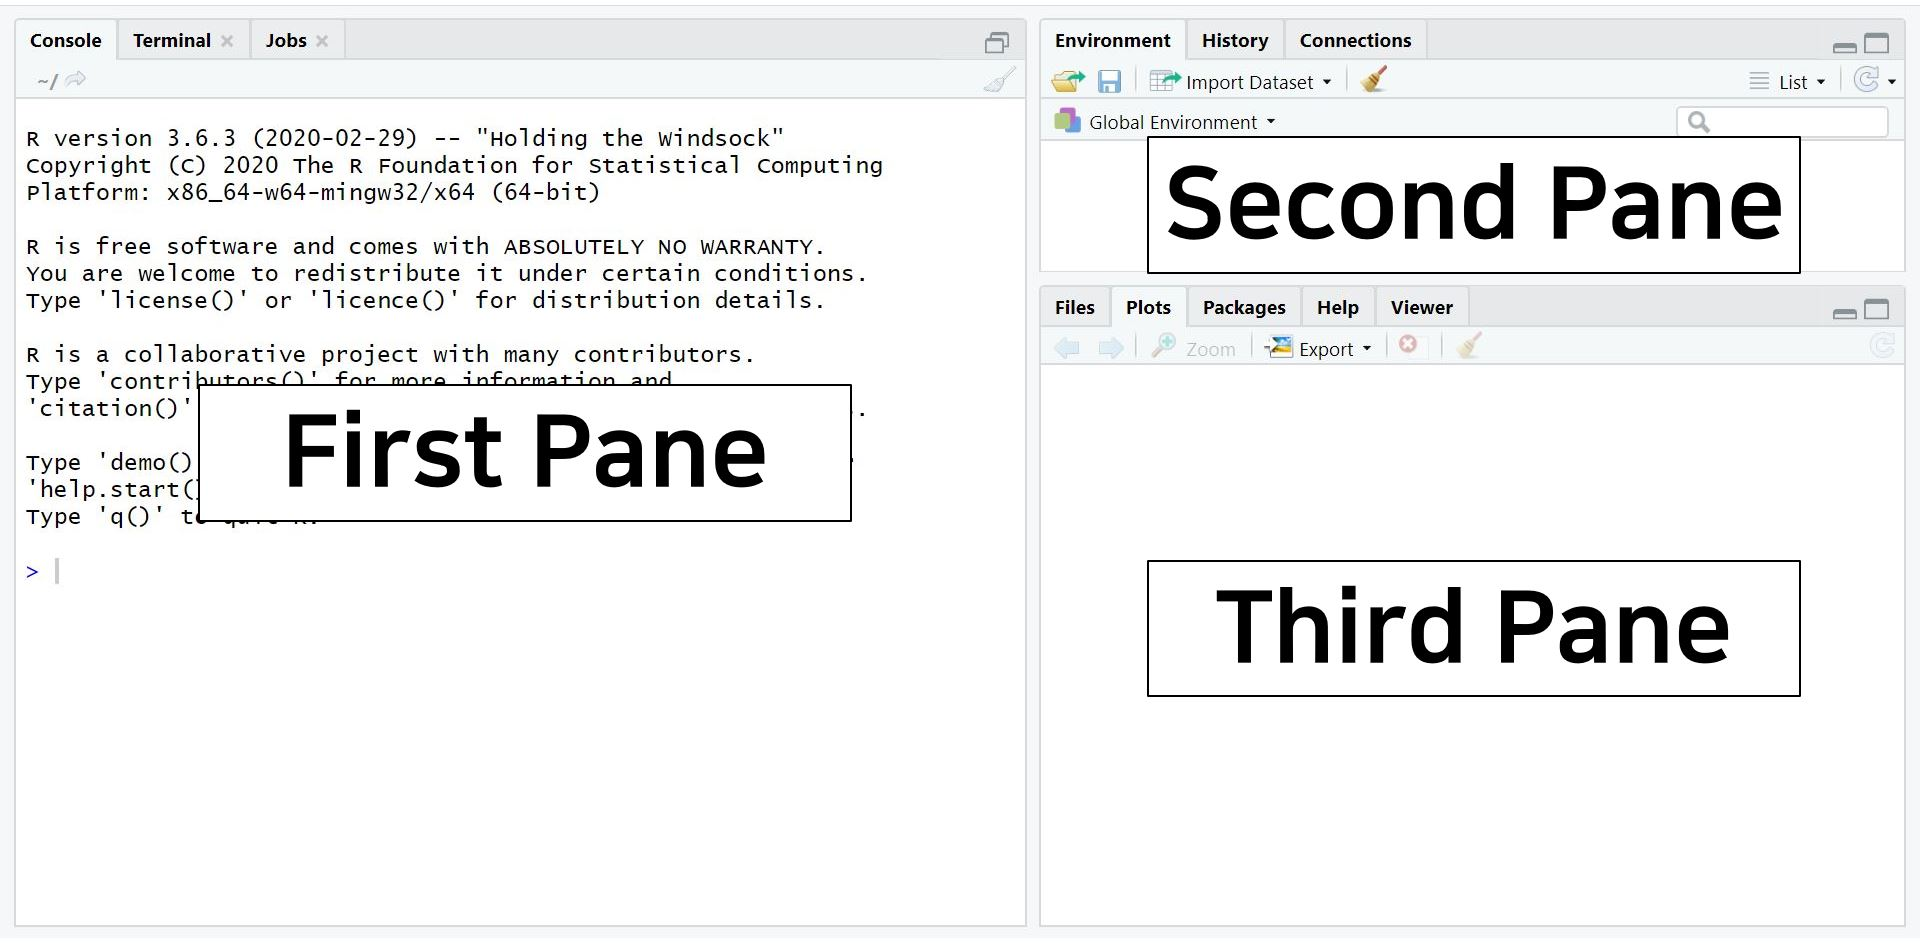
\includegraphics{./img/first_glance.jpg}

\subsection{Open a new R script}\label{open-a-new-r-script}

\begin{itemize}
\tightlist
\item
  Can you find four panes?
\end{itemize}

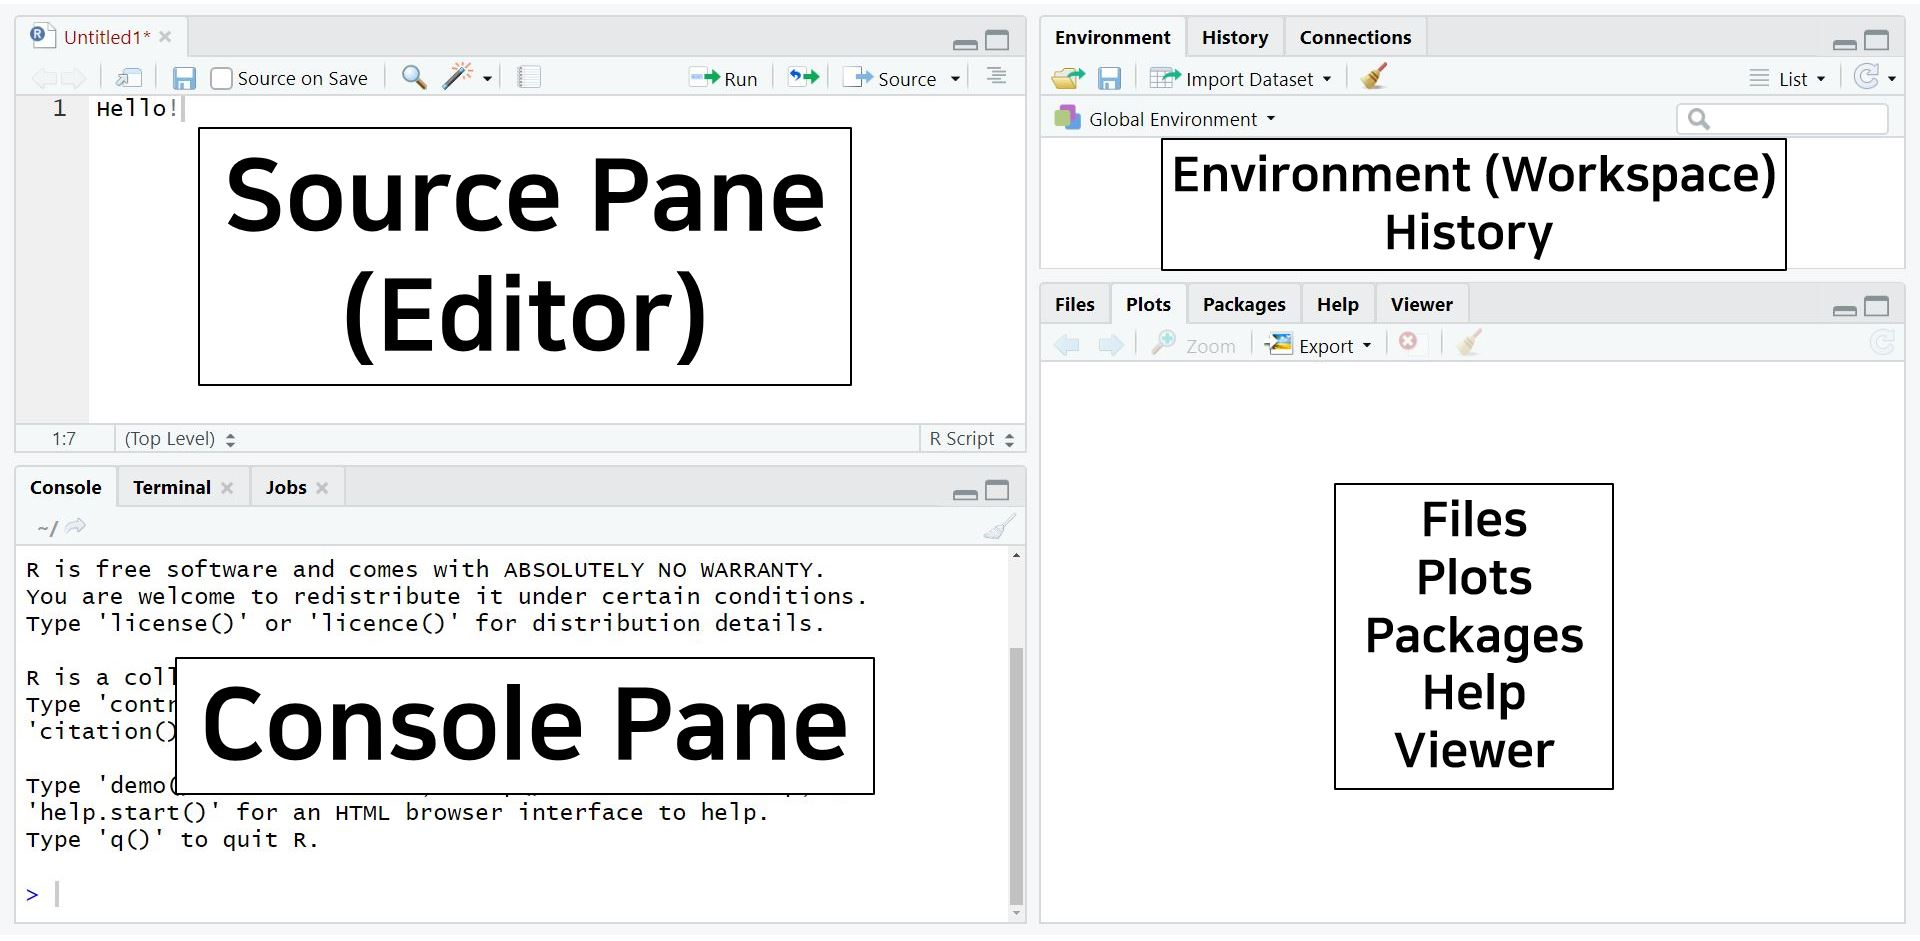
\includegraphics{./img/second_glance.jpg}

\subsection{Individualize R}\label{individualize-r}

\begin{itemize}
\tightlist
\item
  Can you find your own R style?
\end{itemize}

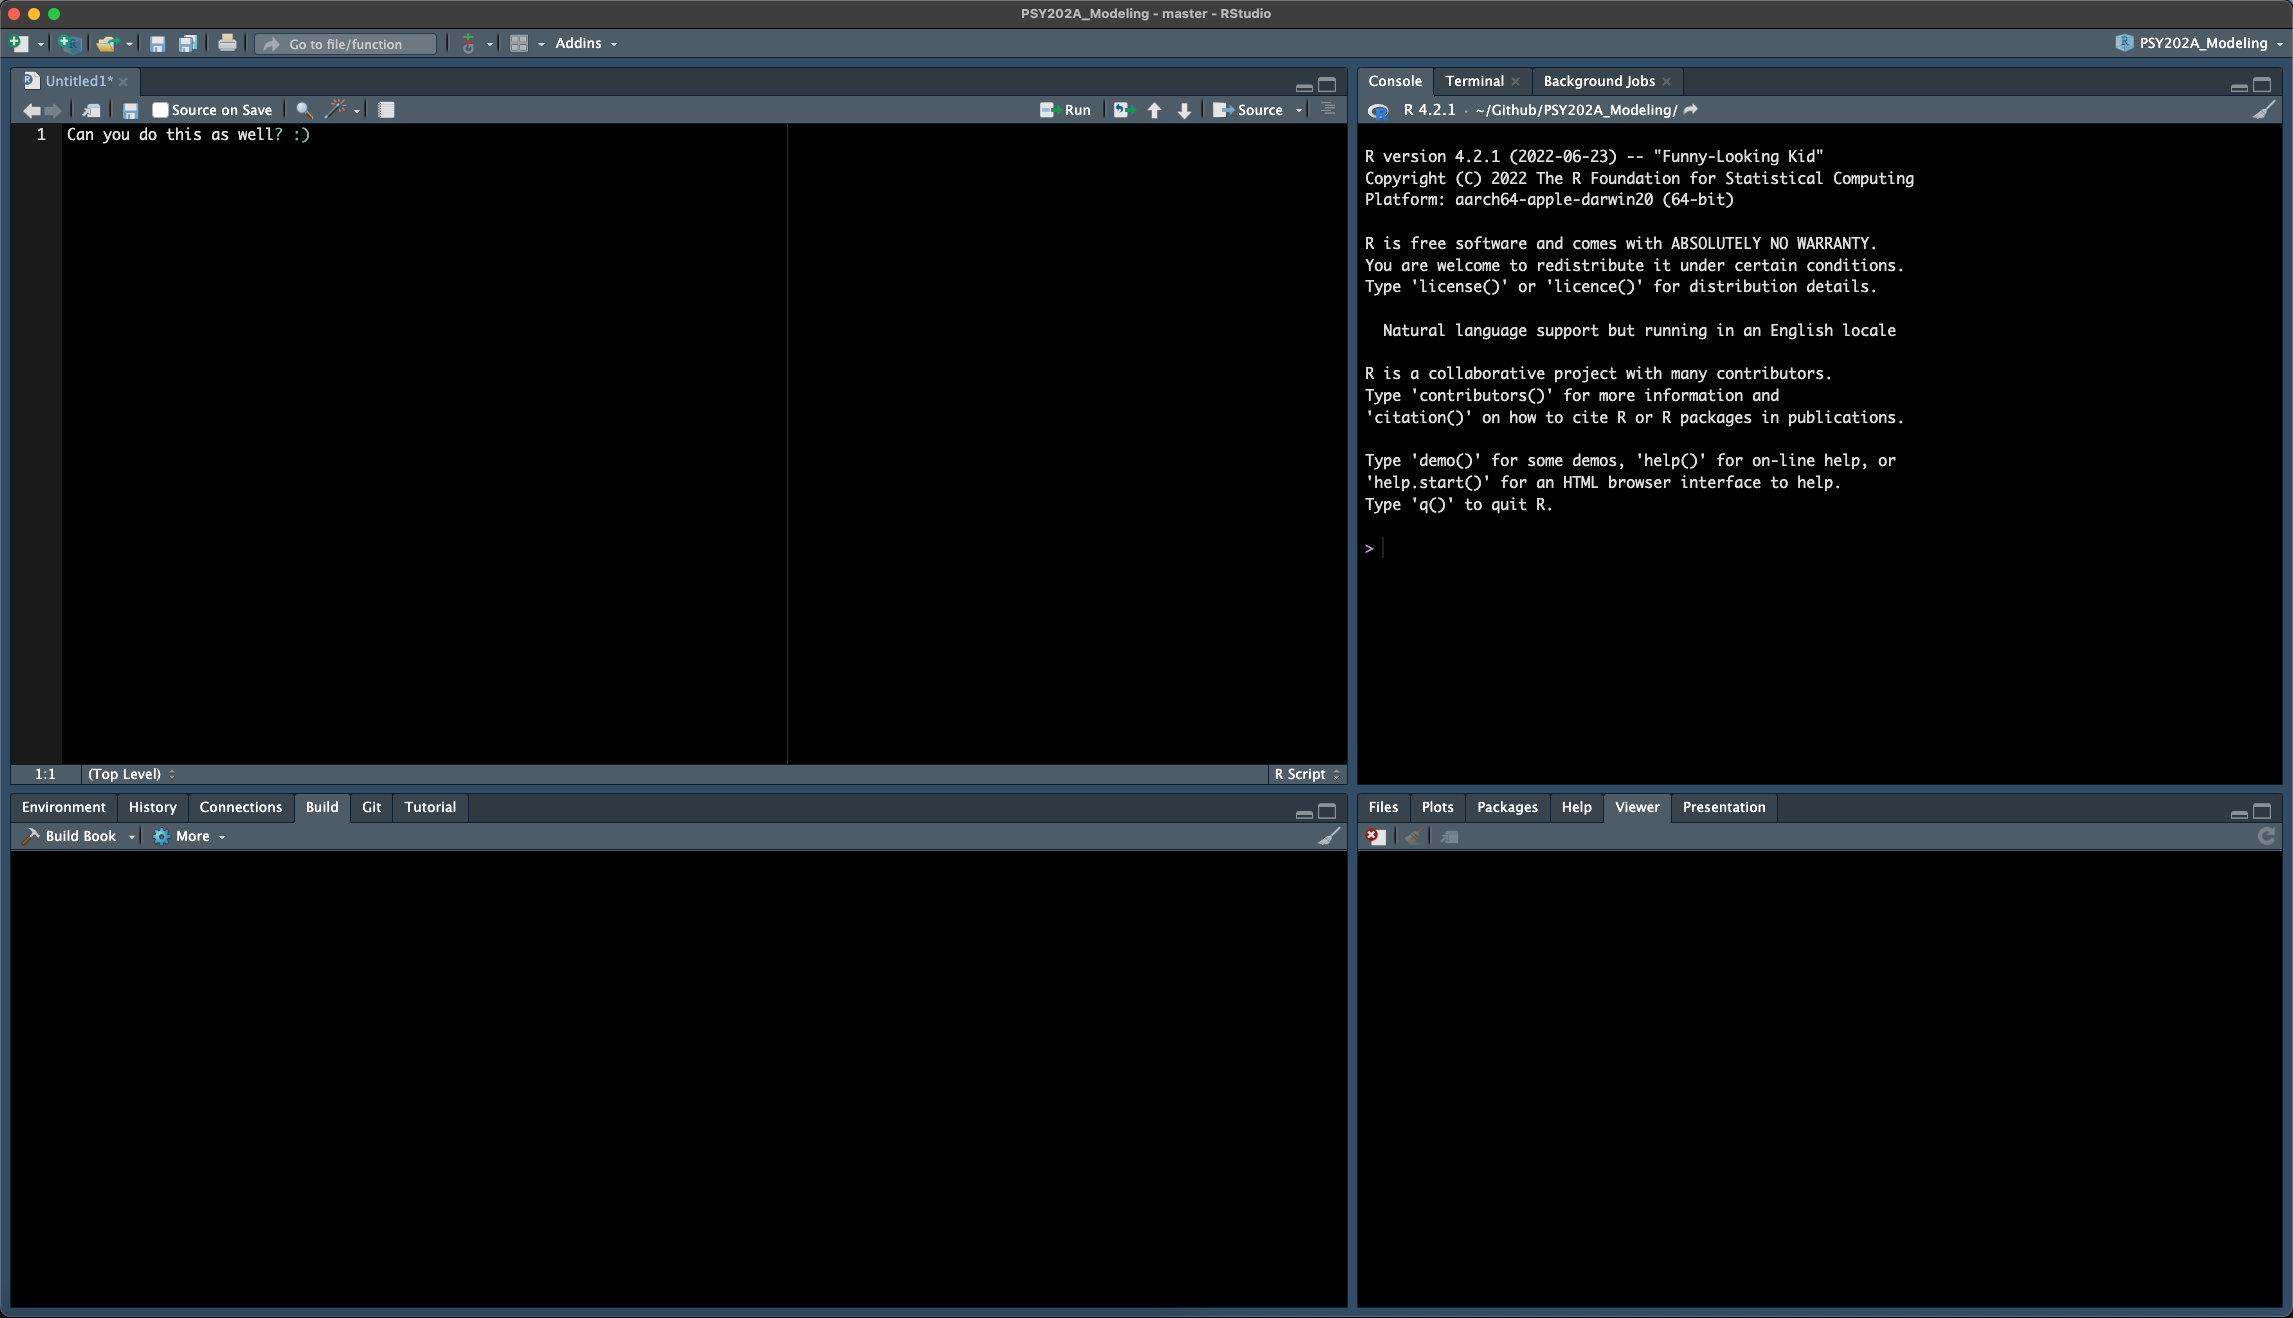
\includegraphics{./img/third_glance.png}

\subsection{Some useful settings}\label{some-useful-settings}

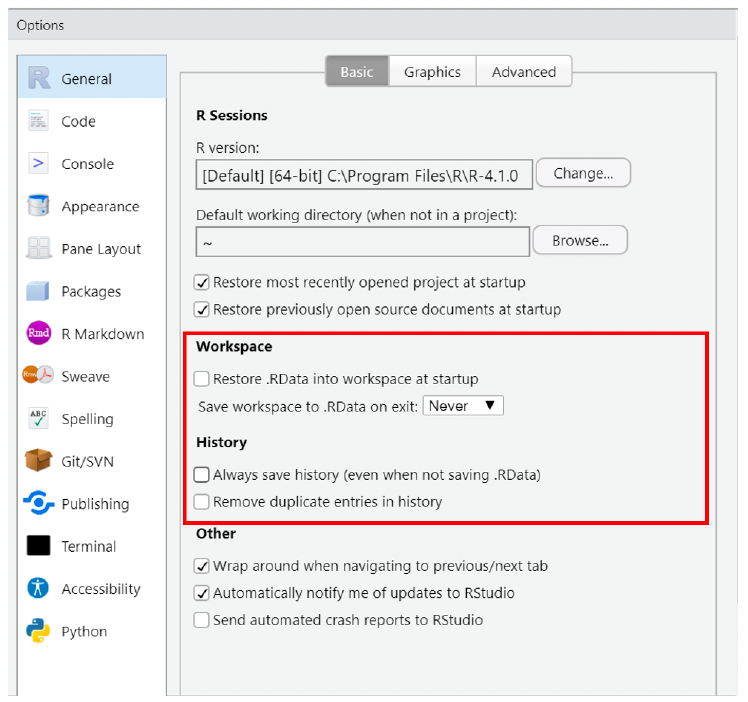
\includegraphics{./img/useful_settings.png}

\begin{itemize}
\tightlist
\item
  Under ``Workspace'':

  \begin{itemize}
  \tightlist
  \item
    Uncheck restore .RData into workspace at startup.
  \item
    Save workshop to .Rdata on exit: ``Never''.
  \end{itemize}
\item
  Under ``History'':

  \begin{itemize}
  \tightlist
  \item
    Uncheck ``Always save history (even when not saving .RData).
  \item
    Uncheck ``Remove duplicate entries in history''.
  \end{itemize}
\end{itemize}

\section{Interacting with R}\label{interacting-with-r}

\begin{itemize}
\tightlist
\item
  How to run R commands?

  \begin{itemize}
  \tightlist
  \item
    Put your cursor on a line, or select the line(s), hit the Run button.
  \item
    The hot key for Run the current line'selection is Ctrl + Enter (Windoes) or Command + Return (Mac).
  \end{itemize}
\item
  Can you run the below code?
\end{itemize}

\begin{Shaded}
\begin{Highlighting}[]
\NormalTok{greetings }\OtherTok{\textless{}{-}} \StringTok{"Hello PSY202A"}
\FunctionTok{print}\NormalTok{(greetings)}
\end{Highlighting}
\end{Shaded}

\begin{itemize}
\item
  Everything starting with a pound sign (\#) is considered as a comment. R will skep all the characters after \# until it finds a new line of command.
\item
  Can you run the below code?
\end{itemize}

\begin{Shaded}
\begin{Highlighting}[]
\NormalTok{Comment}

\CommentTok{\# Comment}
\end{Highlighting}
\end{Shaded}

\section{Numerical computation}\label{numerical-computation}

\subsection{Using R as a numerical calculator}\label{using-r-as-a-numerical-calculator}

\begin{itemize}
\tightlist
\item
  Can you run the code below?
\end{itemize}

\begin{Shaded}
\begin{Highlighting}[]
\DecValTok{2} \SpecialCharTok{+} \DecValTok{4} \CommentTok{\# Addition}
\DecValTok{2} \SpecialCharTok{{-}} \DecValTok{4} \CommentTok{\# Subtraction}
\DecValTok{2} \SpecialCharTok{*} \DecValTok{4} \CommentTok{\# Multiplication}
\DecValTok{2} \SpecialCharTok{/} \DecValTok{4} \CommentTok{\# Division}
\DecValTok{2} \SpecialCharTok{**} \DecValTok{4} \CommentTok{\# Power}
\FunctionTok{sqrt}\NormalTok{(}\DecValTok{144}\NormalTok{) }\CommentTok{\# Square root}
\FunctionTok{log}\NormalTok{(}\DecValTok{144}\NormalTok{) }\CommentTok{\# Natural logarithm}
\FunctionTok{exp}\NormalTok{(}\DecValTok{5}\NormalTok{) }\CommentTok{\# Exponential, i.e., power of e}
\NormalTok{(}\DecValTok{10} \SpecialCharTok{+} \DecValTok{2}\SpecialCharTok{*}\FunctionTok{log}\NormalTok{(}\DecValTok{8}\NormalTok{) }\SpecialCharTok{{-}}\NormalTok{ (}\FunctionTok{exp}\NormalTok{(}\DecValTok{8}\NormalTok{) }\SpecialCharTok{{-}} \DecValTok{4}\NormalTok{)}\SpecialCharTok{/}\DecValTok{3}\NormalTok{) }\SpecialCharTok{*} \DecValTok{7}
\end{Highlighting}
\end{Shaded}

\begin{itemize}
\tightlist
\item
  Here, \texttt{sqrt()}, \texttt{log()}, and \texttt{exp()} are numerical functions.
\end{itemize}

\subsubsection{Exercise: Numerical calculator}\label{exercise-numerical-calculator}

\begin{itemize}
\tightlist
\item
  Can you give me the answer to the mathematical formula below?
\end{itemize}

\[
\frac{26}{\text{log}(5)}\times e^{3} + (-0.2)
\]

\begin{itemize}
\tightlist
\item
  How about this?
\end{itemize}

\[
-\sqrt( \text{ln}7 )
\]

\subsection{Using R as a logical calculator}\label{using-r-as-a-logical-calculator}

\begin{itemize}
\tightlist
\item
  You can also use R for logical statements.
\end{itemize}

\begin{Shaded}
\begin{Highlighting}[]
\DecValTok{1} \SpecialCharTok{==} \DecValTok{1} \CommentTok{\# equal}
\DecValTok{1} \SpecialCharTok{!=} \DecValTok{2} \CommentTok{\# unequal}
\DecValTok{10} \SpecialCharTok{\textgreater{}} \DecValTok{1} \CommentTok{\# greater than}
\DecValTok{10} \SpecialCharTok{\textgreater{}=} \DecValTok{1} \CommentTok{\# greater than or equal to}
\end{Highlighting}
\end{Shaded}

\subsubsection{Exercise: Logical calculator}\label{exercise-logical-calculator}

\begin{itemize}
\tightlist
\item
  Then\ldots{} can you program your code to evaluate the below statements?

  \begin{itemize}
  \tightlist
  \item
    Try this first: 5 is lower than or equal to 10. What is the result? Does this make sense?
  \item
    Then, try this second: 10 is not equal to 10. What is the result? Does this make sense?
  \end{itemize}
\end{itemize}

\section{Types of objects}\label{types-of-objects}

\begin{itemize}
\tightlist
\item
  In R, anything with a name is an object.

  \begin{itemize}
  \tightlist
  \item
    You can give an object with any name you want insofar as that name is not taken in R already.
  \end{itemize}
\item
  An object can contain more than one value and have more complex data strutures, such as:

  \begin{itemize}
  \tightlist
  \item
    vector: a series of values of the same data type
  \item
    matrix: a two-dimensional table of values with the same data type
  \item
    data frame: a two-dimensional table of values, may not be the same data type
  \item
    list: an object made of objects
  \end{itemize}
\end{itemize}

\subsection{Vector: Intro}\label{vector-intro}

\begin{itemize}
\tightlist
\item
  The concatenate function \texttt{c()} is usually used to put a set of values together.

  \begin{itemize}
  \tightlist
  \item
    An object \texttt{iq} is a vector of 5 IQ scores.
  \end{itemize}
\end{itemize}

\begin{Shaded}
\begin{Highlighting}[]
\CommentTok{\# A vector of IQ scores}
\NormalTok{iq }\OtherTok{\textless{}{-}} \FunctionTok{c}\NormalTok{(}\DecValTok{90}\NormalTok{, }\DecValTok{100}\NormalTok{, }\DecValTok{105}\NormalTok{, }\DecValTok{110}\NormalTok{, }\DecValTok{95}\NormalTok{)}

\CommentTok{\# Here, \textquotesingle{}iq\textquotesingle{} is an object}

\CommentTok{\# Print the IQ object}
\FunctionTok{print}\NormalTok{(iq)}
\NormalTok{iq}
\end{Highlighting}
\end{Shaded}

\begin{itemize}
\tightlist
\item
  Out of curiosity, what should we do if we want to know the sum of all the five iq scores? You can use the \texttt{sum()} function. Can you try?
\end{itemize}

\begin{Shaded}
\begin{Highlighting}[]
\CommentTok{\# Hint: put an object name within the sum()}
\end{Highlighting}
\end{Shaded}

\begin{itemize}
\tightlist
\item
  Many other functions also return vectors as results.

  \begin{itemize}
  \tightlist
  \item
    For instance, the sequence operator (:) generates consecutive numbers.
  \end{itemize}
\end{itemize}

\begin{Shaded}
\begin{Highlighting}[]
\NormalTok{numbers }\OtherTok{\textless{}{-}} \DecValTok{1}\SpecialCharTok{:}\DecValTok{100}
\NormalTok{numbers}
\end{Highlighting}
\end{Shaded}

\subsubsection{Exercise: Vector intro}\label{exercise-vector-intro}

\begin{itemize}
\tightlist
\item
  There are other specific functions. Can you guess what each of the functions does?
\end{itemize}

\begin{Shaded}
\begin{Highlighting}[]
\CommentTok{\# Describe what the below function does: }
\NormalTok{values\_1 }\OtherTok{\textless{}{-}} \FunctionTok{seq}\NormalTok{(}\DecValTok{1}\NormalTok{, }\DecValTok{5}\NormalTok{, }\AttributeTok{by =} \DecValTok{1}\NormalTok{)}

\CommentTok{\# Describe what the below function does: }
\NormalTok{values\_2 }\OtherTok{\textless{}{-}} \FunctionTok{seq}\NormalTok{(}\DecValTok{1}\NormalTok{, }\DecValTok{5}\NormalTok{, }\AttributeTok{by =} \FloatTok{0.5}\NormalTok{)}

\CommentTok{\# Describe what the below function does: }
\NormalTok{values\_3 }\OtherTok{\textless{}{-}} \FunctionTok{rep}\NormalTok{(}\DecValTok{1}\NormalTok{, }\DecValTok{5}\NormalTok{)}

\CommentTok{\# Describe what the below function does: }
\NormalTok{values\_4 }\OtherTok{\textless{}{-}} \FunctionTok{rep}\NormalTok{(}\DecValTok{1}\SpecialCharTok{:}\DecValTok{5}\NormalTok{, }\DecValTok{3}\NormalTok{)}
\end{Highlighting}
\end{Shaded}

\subsection{Vector: Advanced}\label{vector-advanced}

\begin{itemize}
\item
  There are a couple of distribution functions that can be used to generate a vector of random numbers from a specific distribution.
\item
  For example, you can generate 5 random numbers from a normal distribution with a mean of 0 and a standard deviation of 1:
\end{itemize}

\begin{Shaded}
\begin{Highlighting}[]
\NormalTok{random\_normal }\OtherTok{\textless{}{-}} \FunctionTok{rnorm}\NormalTok{(}\DecValTok{5}\NormalTok{, }\DecValTok{0}\NormalTok{, }\DecValTok{1}\NormalTok{)}
\NormalTok{random\_normal}
\end{Highlighting}
\end{Shaded}

\begin{itemize}
\tightlist
\item
  As another example, you can generate 5 random numbers from a uniform distribution between 0 and 1:
\end{itemize}

\begin{Shaded}
\begin{Highlighting}[]
\NormalTok{random\_uniform }\OtherTok{\textless{}{-}} \FunctionTok{runif}\NormalTok{(}\DecValTok{5}\NormalTok{, }\DecValTok{0}\NormalTok{, }\DecValTok{1}\NormalTok{)}
\NormalTok{random\_uniform}
\end{Highlighting}
\end{Shaded}

\begin{itemize}
\tightlist
\item
  The standard arithmetic operators and functions apply to vectors on a element-wise basis.
\end{itemize}

\begin{Shaded}
\begin{Highlighting}[]
\NormalTok{A }\OtherTok{\textless{}{-}} \FunctionTok{c}\NormalTok{(}\DecValTok{1}\NormalTok{, }\DecValTok{2}\NormalTok{, }\DecValTok{3}\NormalTok{, }\DecValTok{4}\NormalTok{) }\SpecialCharTok{{-}} \DecValTok{4}
\NormalTok{A}

\NormalTok{B }\OtherTok{\textless{}{-}} \FunctionTok{c}\NormalTok{(}\DecValTok{1}\NormalTok{, }\DecValTok{2}\NormalTok{, }\DecValTok{3}\NormalTok{, }\DecValTok{4}\NormalTok{)}\SpecialCharTok{/}\DecValTok{4}
\NormalTok{B}

\NormalTok{C }\OtherTok{\textless{}{-}} \FunctionTok{c}\NormalTok{(}\DecValTok{1}\NormalTok{, }\DecValTok{2}\NormalTok{, }\DecValTok{3}\NormalTok{, }\DecValTok{4}\NormalTok{)}\SpecialCharTok{/}\FunctionTok{c}\NormalTok{(}\DecValTok{4}\NormalTok{, }\DecValTok{3}\NormalTok{, }\DecValTok{2}\NormalTok{, }\DecValTok{1}\NormalTok{)}
\NormalTok{C}

\NormalTok{D }\OtherTok{\textless{}{-}} \FunctionTok{log}\NormalTok{(}\FunctionTok{c}\NormalTok{(}\DecValTok{1}\NormalTok{, }\DecValTok{2}\NormalTok{, }\DecValTok{3}\NormalTok{, }\DecValTok{4}\NormalTok{))}
\NormalTok{D}
\end{Highlighting}
\end{Shaded}

\begin{itemize}
\tightlist
\item
  All elements in a vector must be the same type

  \begin{itemize}
  \tightlist
  \item
    Numeric, character (aka. string), logic
  \end{itemize}
\end{itemize}

\begin{Shaded}
\begin{Highlighting}[]
\NormalTok{numeric\_vector }\OtherTok{\textless{}{-}} \FunctionTok{c}\NormalTok{(}\DecValTok{1}\NormalTok{, }\DecValTok{2}\NormalTok{, }\DecValTok{3}\NormalTok{, }\DecValTok{4}\NormalTok{)}

\NormalTok{character\_vector }\OtherTok{\textless{}{-}} \FunctionTok{c}\NormalTok{(}\StringTok{"developmental"}\NormalTok{, }\StringTok{"health"}\NormalTok{, }\StringTok{"quantitative"}\NormalTok{)}

\NormalTok{logical\_vector }\OtherTok{\textless{}{-}} \FunctionTok{c}\NormalTok{(}\ConstantTok{FALSE}\NormalTok{, }\ConstantTok{TRUE}\NormalTok{, }\ConstantTok{FALSE}\NormalTok{, }\ConstantTok{FALSE}\NormalTok{)}
\end{Highlighting}
\end{Shaded}

\subsubsection{Exercise: Vector advanced}\label{exercise-vector-advanced}

Can you run the code below? What do you see?

\begin{Shaded}
\begin{Highlighting}[]
\NormalTok{numeric\_vector}\SpecialCharTok{\^{}}\DecValTok{2}

\DecValTok{1}\SpecialCharTok{/}\NormalTok{numeric\_vector}

\NormalTok{numeric\_vector }\SpecialCharTok{+}\NormalTok{ character\_vector}

\NormalTok{character\_vector }\SpecialCharTok{+}\NormalTok{ logical\_vector}

\NormalTok{numeric\_vector }\SpecialCharTok{+}\NormalTok{ logical\_vector}

\NormalTok{logical\_vector }\SpecialCharTok{+}\NormalTok{ logical\_vector}

\NormalTok{logical\_vector}\SpecialCharTok{+}\DecValTok{5}
\end{Highlighting}
\end{Shaded}

\subsection{Matrix: intro}\label{matrix-intro}

\begin{itemize}
\tightlist
\item
  We can create a matrix by combining multiple vectors (e.g., perhaps associated with multiple scales)
\end{itemize}

\begin{Shaded}
\begin{Highlighting}[]
\NormalTok{scale1 }\OtherTok{\textless{}{-}} \FunctionTok{c}\NormalTok{(}\DecValTok{1}\NormalTok{, }\DecValTok{4}\NormalTok{, }\DecValTok{7}\NormalTok{, }\DecValTok{4}\NormalTok{, }\DecValTok{5}\NormalTok{)}
\NormalTok{scale2 }\OtherTok{\textless{}{-}} \FunctionTok{c}\NormalTok{(}\DecValTok{5}\NormalTok{, }\DecValTok{6}\NormalTok{, }\DecValTok{8}\NormalTok{, }\DecValTok{3}\NormalTok{, }\DecValTok{2}\NormalTok{)}
\NormalTok{scale3 }\OtherTok{\textless{}{-}} \FunctionTok{c}\NormalTok{(}\DecValTok{0}\NormalTok{, }\DecValTok{9}\NormalTok{, }\DecValTok{8}\NormalTok{, }\DecValTok{9}\NormalTok{, }\DecValTok{3}\NormalTok{)}
\end{Highlighting}
\end{Shaded}

\begin{itemize}
\tightlist
\item
  We could arrange these into a table, using \texttt{cbind()} function (bind by column).
\end{itemize}

\begin{Shaded}
\begin{Highlighting}[]
\NormalTok{my\_data }\OtherTok{\textless{}{-}} \FunctionTok{cbind}\NormalTok{(scale1, scale2, scale3)}
\NormalTok{my\_data}
\end{Highlighting}
\end{Shaded}

\begin{itemize}
\tightlist
\item
  Or, if our data were in one long vector:
\end{itemize}

\begin{Shaded}
\begin{Highlighting}[]
\NormalTok{long\_vec }\OtherTok{\textless{}{-}} \FunctionTok{c}\NormalTok{(scale1, scale2, scale3)}
\NormalTok{my\_matrix }\OtherTok{\textless{}{-}} \FunctionTok{matrix}\NormalTok{(long\_vec, }\AttributeTok{ncol =} \DecValTok{3}\NormalTok{, }\AttributeTok{byrow =} \ConstantTok{FALSE}\NormalTok{)}
\NormalTok{my\_matrix}
\end{Highlighting}
\end{Shaded}

\subsection{Matrix: advanced}\label{matrix-advanced}

\begin{itemize}
\tightlist
\item
  Find the size of the matrix (i.e., the number of rows and the number of columns) using \texttt{dim()}:
\end{itemize}

\begin{Shaded}
\begin{Highlighting}[]
\FunctionTok{dim}\NormalTok{(my\_matrix)}
\end{Highlighting}
\end{Shaded}

\begin{itemize}
\tightlist
\item
  ,where this parallels \texttt{length()} for vectors:
\end{itemize}

\begin{Shaded}
\begin{Highlighting}[]
\FunctionTok{length}\NormalTok{(scale1)}
\end{Highlighting}
\end{Shaded}

\subsubsection{Exercise: matrix advanced}\label{exercise-matrix-advanced}

\begin{itemize}
\item
  Can you create an arbitrary matrix with 5 rows and 3 columns? You can do anything to achieve this goal.
\item
  If you are successful, can you transpose the matrix using the \texttt{t()} function?
\item
  What is the size of the transposed matrix?
\end{itemize}

\subsection{Data frame}\label{data-frame}

\begin{itemize}
\tightlist
\item
  Similar to matrices, data frames can be created by combining multiple vectors, but data frames allow for different vector types (e.g., number, character, logical), but preserves the characteristics of each type.
\end{itemize}

\begin{Shaded}
\begin{Highlighting}[]
\NormalTok{v1 }\OtherTok{\textless{}{-}} \DecValTok{1001}\SpecialCharTok{:}\DecValTok{1006}
\NormalTok{v2 }\OtherTok{\textless{}{-}} \FunctionTok{c}\NormalTok{(}\FloatTok{407.56}\NormalTok{, }\FloatTok{442.20}\NormalTok{, }\FloatTok{385.85}\NormalTok{, }\FloatTok{295.31}\NormalTok{, }\FloatTok{408.10}\NormalTok{, }\FloatTok{280.52}\NormalTok{)}
\NormalTok{v3 }\OtherTok{\textless{}{-}} \FunctionTok{c}\NormalTok{(}\StringTok{"A"}\NormalTok{, }\StringTok{"A"}\NormalTok{, }\StringTok{"A"}\NormalTok{, }\StringTok{"B"}\NormalTok{, }\StringTok{"B"}\NormalTok{, }\StringTok{"B"}\NormalTok{)}

\NormalTok{my\_dataframe }\OtherTok{\textless{}{-}} \FunctionTok{data.frame}\NormalTok{(}\AttributeTok{id =}\NormalTok{ v1, }\AttributeTok{reactiontime=}\NormalTok{ v2, }\AttributeTok{condition =}\NormalTok{ v3)}
\NormalTok{my\_dataframe}
\end{Highlighting}
\end{Shaded}

\subsubsection{Exercise: data frame}\label{exercise-data-frame}

\begin{itemize}
\tightlist
\item
  Can you describe the differences between a matrix and a data frame in R?
\end{itemize}

\subsection{List}\label{list}

\begin{itemize}
\tightlist
\item
  Data frames must be rectangular, what if our data are non-rectangular?
\end{itemize}

\begin{Shaded}
\begin{Highlighting}[]
\NormalTok{mod\_A }\OtherTok{\textless{}{-}} \FunctionTok{c}\NormalTok{(}\FloatTok{4.25}\NormalTok{, }\FloatTok{2.36}\NormalTok{, }\FloatTok{2.37}\NormalTok{)}
\NormalTok{mod\_B }\OtherTok{\textless{}{-}} \FunctionTok{c}\NormalTok{(}\FloatTok{4.26}\NormalTok{, }\FloatTok{2.45}\NormalTok{, }\FloatTok{2.31}\NormalTok{, }\FloatTok{7.5}\NormalTok{)}
\NormalTok{mod\_C }\OtherTok{\textless{}{-}} \FunctionTok{c}\NormalTok{(}\FloatTok{4.21}\NormalTok{, }\FloatTok{2.44}\NormalTok{, }\FloatTok{2.29}\NormalTok{, }\FloatTok{7.7}\NormalTok{, }\FloatTok{4.1}\NormalTok{)}
\NormalTok{flag }\OtherTok{\textless{}{-}} \FunctionTok{c}\NormalTok{(}\ConstantTok{FALSE}\NormalTok{, }\ConstantTok{FALSE}\NormalTok{, }\ConstantTok{TRUE}\NormalTok{)}
\end{Highlighting}
\end{Shaded}

\begin{itemize}
\tightlist
\item
  A list will allow any set of R objects to be combined into a single object
\end{itemize}

\begin{Shaded}
\begin{Highlighting}[]
\NormalTok{my\_list }\OtherTok{\textless{}{-}} \FunctionTok{list}\NormalTok{(}\AttributeTok{parA =}\NormalTok{ mod\_A, }\AttributeTok{parB =}\NormalTok{ mod\_C, }\AttributeTok{parC =}\NormalTok{ mod\_C, }\AttributeTok{flag =}\NormalTok{ flag)}
\NormalTok{my\_list}
\end{Highlighting}
\end{Shaded}

\subsection{Exercise: Selecting elements in objects}\label{exercise-selecting-elements-in-objects}

\begin{itemize}
\item
  We can select elements of vectors, matrices, data frames, and lists using brackets (i.e., {[}{]}).
\item
  For each chunk of the code below, think of the expected output before running the code, and see if your guess was correct after running the code:
\end{itemize}

\subsubsection{For vectors}\label{for-vectors}

\begin{itemize}
\tightlist
\item
  Given the vector below:
\end{itemize}

\begin{Shaded}
\begin{Highlighting}[]
\NormalTok{scale1 }\OtherTok{\textless{}{-}} \FunctionTok{c}\NormalTok{(}\DecValTok{1}\NormalTok{, }\DecValTok{4}\NormalTok{, }\DecValTok{7}\NormalTok{, }\DecValTok{4}\NormalTok{, }\DecValTok{5}\NormalTok{)}
\end{Highlighting}
\end{Shaded}

\begin{itemize}
\tightlist
\item
  Can you expect the outcome?
\end{itemize}

\begin{Shaded}
\begin{Highlighting}[]
\NormalTok{scale1[}\DecValTok{3}\NormalTok{]}
\end{Highlighting}
\end{Shaded}

\subsubsection{For matrices}\label{for-matrices}

\begin{itemize}
\tightlist
\item
  Recall that this is our predefined matrix object:
\end{itemize}

\begin{Shaded}
\begin{Highlighting}[]
\NormalTok{my\_matrix}
\end{Highlighting}
\end{Shaded}

\begin{itemize}
\tightlist
\item
  Can you expect the outcome?
\end{itemize}

\begin{Shaded}
\begin{Highlighting}[]
\NormalTok{my\_matrix[ , }\DecValTok{2}\NormalTok{]}
\NormalTok{my\_matrix[}\DecValTok{1}\NormalTok{,  ]}
\NormalTok{my\_matrix[}\DecValTok{1}\NormalTok{, }\DecValTok{2}\NormalTok{]}
\NormalTok{my\_matrix[}\DecValTok{1}\SpecialCharTok{:}\DecValTok{2}\NormalTok{,  ]}
\NormalTok{my\_matrix[ , }\DecValTok{1}\SpecialCharTok{:}\DecValTok{2}\NormalTok{]}
\end{Highlighting}
\end{Shaded}

\subsubsection{For data frames}\label{for-data-frames}

\begin{itemize}
\tightlist
\item
  Recall that this is our predefined data frame object:
\end{itemize}

\begin{Shaded}
\begin{Highlighting}[]
\NormalTok{my\_dataframe}
\end{Highlighting}
\end{Shaded}

\begin{itemize}
\tightlist
\item
  Can you expect the outcome?
\end{itemize}

\begin{Shaded}
\begin{Highlighting}[]
\NormalTok{my\_dataframe[}\DecValTok{1}\NormalTok{, }\DecValTok{1}\NormalTok{]}
\NormalTok{my\_dataframe[}\DecValTok{1}\SpecialCharTok{:}\DecValTok{2}\NormalTok{,  ]}
\NormalTok{my\_dataframe[ , }\DecValTok{1}\SpecialCharTok{:}\DecValTok{2}\NormalTok{]}
\NormalTok{my\_dataframe}\SpecialCharTok{$}\NormalTok{id}
\end{Highlighting}
\end{Shaded}

\subsubsection{For lists}\label{for-lists}

\begin{itemize}
\tightlist
\item
  Recall that this is our predefined list object:
\end{itemize}

\begin{Shaded}
\begin{Highlighting}[]
\NormalTok{my\_list}
\end{Highlighting}
\end{Shaded}

\begin{itemize}
\tightlist
\item
  Can you expect the outcome?

  \begin{itemize}
  \tightlist
  \item
    Note that, for list objects, we sometimes need to use the double brackets to extract an element of a part of a list
  \end{itemize}
\end{itemize}

\begin{Shaded}
\begin{Highlighting}[]
\NormalTok{my\_list[}\DecValTok{1}\NormalTok{]}
\NormalTok{my\_list[[}\DecValTok{1}\NormalTok{]]}
\NormalTok{my\_list[}\DecValTok{2}\NormalTok{]}
\NormalTok{my\_list[[}\DecValTok{2}\NormalTok{]]}
\NormalTok{my\_list}\SpecialCharTok{$}\NormalTok{parB}
\end{Highlighting}
\end{Shaded}

\subsubsection{Another bonus exercise for you}\label{another-bonus-exercise-for-you}

\begin{itemize}
\tightlist
\item
  Create a new data frame using the following vectors:
\end{itemize}

\begin{Shaded}
\begin{Highlighting}[]
\NormalTok{id }\OtherTok{\textless{}{-}} \FunctionTok{c}\NormalTok{(}\DecValTok{1001}\SpecialCharTok{:}\DecValTok{1040}\NormalTok{)}
\NormalTok{x }\OtherTok{\textless{}{-}} \FunctionTok{runif}\NormalTok{(}\DecValTok{40}\NormalTok{, }\DecValTok{250}\NormalTok{, }\DecValTok{500}\NormalTok{)}
\NormalTok{y }\OtherTok{\textless{}{-}}\NormalTok{ x }\SpecialCharTok{*} \FloatTok{0.2} \SpecialCharTok{+} \FunctionTok{runif}\NormalTok{(}\DecValTok{40}\NormalTok{, }\DecValTok{200}\NormalTok{, }\DecValTok{450}\NormalTok{)}
\NormalTok{gender }\OtherTok{\textless{}{-}} \FunctionTok{sample}\NormalTok{(}\FunctionTok{c}\NormalTok{(}\StringTok{"M"}\NormalTok{, }\StringTok{"F"}\NormalTok{), }\DecValTok{40}\NormalTok{, }\AttributeTok{replace =} \ConstantTok{TRUE}\NormalTok{)}
\end{Highlighting}
\end{Shaded}

\begin{itemize}
\tightlist
\item
  Get the mean of y in the data frame you just created. (Hint: use \$ to extract the variable; use function
  mean() to compute the mean.)
\end{itemize}

\section{Workspace}\label{workspace}

\begin{itemize}
\tightlist
\item
  Recall that everything that has a name in R is called an object.
\item
  The workspace is your current R working environment and includes every user-defined objects, such as vectors, matrices, data frames, lists, etc.
\item
  The ls() function will list all the objects in a workspace.
\item
  The object(s) can be removed from the workspace by the \texttt{rm()} function.
\end{itemize}

\subsection{Functions to manage workspace}\label{functions-to-manage-workspace}

\begin{itemize}
\tightlist
\item
  Can you run the code below and see what happens? Can you understand what is happening?
\end{itemize}

\begin{Shaded}
\begin{Highlighting}[]
\FunctionTok{ls}\NormalTok{()}
\end{Highlighting}
\end{Shaded}

\begin{itemize}
\tightlist
\item
  What about this? What happened?
\end{itemize}

\begin{Shaded}
\begin{Highlighting}[]
\FunctionTok{rm}\NormalTok{(v1)}
\FunctionTok{ls}\NormalTok{()}
\end{Highlighting}
\end{Shaded}

\begin{itemize}
\tightlist
\item
  Shall we remove all the objects?
\end{itemize}

\begin{Shaded}
\begin{Highlighting}[]
\CommentTok{\# Remove all the objects in the workspace}
\FunctionTok{rm}\NormalTok{(}\AttributeTok{list=}\FunctionTok{ls}\NormalTok{(}\AttributeTok{all =} \ConstantTok{TRUE}\NormalTok{))}
\end{Highlighting}
\end{Shaded}

\begin{itemize}
\tightlist
\item
  If you haven't unchecked the box about Workspace in the Global Options, at the end of an R session, you will be asked whether you want to save an image of the current workspace that is automatically reloaded the next time R is started. Choose NO.
\item
  Note that the workspace consists only of R objects, not of any of the output that you have generated during a session (e.g., images). If you want to save your output, just copy it from the console.
\item
  Also, there are ways to export your data and save them in some specific formats for further uses.
\end{itemize}

\section{Working directory}\label{working-directory}

\begin{itemize}
\tightlist
\item
  The working directory is the location (file path) on your computer where R will look for files and where it will save any files.

  \begin{itemize}
  \tightlist
  \item
    For more details, see \url{https://www.rensvandeschoot.com/tutorials/r-for-beginners/}
  \end{itemize}
\item
  To see your current working directory, use \texttt{getwd}:
\end{itemize}

\begin{Shaded}
\begin{Highlighting}[]
\FunctionTok{getwd}\NormalTok{()}
\end{Highlighting}
\end{Shaded}

\begin{itemize}
\item
  You can also check the current working directory by looking at bar at the top of the Console pane.
\item
  To change your working directory, use \texttt{setwd()}:

  \begin{itemize}
  \tightlist
  \item
    For Windows users, \#\# use / instead of\\
  \end{itemize}
\item
  You can also manually set the working directory in the Files tab.
\item
  If you start an R session from a .R file, the default working directory will be set to where the .R file is located on your computer.
\end{itemize}

\section{Importing external data}\label{importing-external-data}

\begin{itemize}
\tightlist
\item
  The most common way is to use the function \texttt{read.table()} to read in .txt files or .dat files; or \texttt{read.csv()} for .csv files.
\end{itemize}

\begin{Shaded}
\begin{Highlighting}[]
\NormalTok{mydata1 }\OtherTok{\textless{}{-}} \FunctionTok{read.table}\NormalTok{(}\AttributeTok{file =} \StringTok{"SAT.dat"}\NormalTok{, }\AttributeTok{header =} \ConstantTok{TRUE}\NormalTok{)}
\FunctionTok{class}\NormalTok{(mydata1)}
\FunctionTok{write.csv}\NormalTok{(mydata1, }\AttributeTok{file =} \StringTok{"SAT.csv"}\NormalTok{, }\AttributeTok{row.names =} \ConstantTok{FALSE}\NormalTok{)}
\end{Highlighting}
\end{Shaded}

\begin{itemize}
\tightlist
\item
  You can try this as well:
\end{itemize}

\begin{Shaded}
\begin{Highlighting}[]
\NormalTok{mydata2 }\OtherTok{\textless{}{-}} \FunctionTok{read.csv}\NormalTok{(}\AttributeTok{file =} \StringTok{"SAT.csv"}\NormalTok{, }\AttributeTok{header =} \ConstantTok{TRUE}\NormalTok{, }\AttributeTok{sep =} \StringTok{","}\NormalTok{)}
\FunctionTok{class}\NormalTok{(mydata2)}
\end{Highlighting}
\end{Shaded}

\begin{itemize}
\tightlist
\item
  You can also manually choose a file to import

  \begin{itemize}
  \tightlist
  \item
    But this will not work for all data formats, so be careful
  \end{itemize}
\end{itemize}

\begin{Shaded}
\begin{Highlighting}[]
\NormalTok{mydata3 }\OtherTok{\textless{}{-}} \FunctionTok{read.table}\NormalTok{(}\FunctionTok{file.choose}\NormalTok{(), }\AttributeTok{header =} \ConstantTok{TRUE}\NormalTok{)}
\FunctionTok{class}\NormalTok{(mydata3)}
\end{Highlighting}
\end{Shaded}

\begin{itemize}
\tightlist
\item
  To look at the whole dataset, directly type the name of it.
\end{itemize}

\begin{Shaded}
\begin{Highlighting}[]
\NormalTok{mydata1}

\NormalTok{mydata2}

\NormalTok{mydata3}
\end{Highlighting}
\end{Shaded}

\begin{itemize}
\tightlist
\item
  To obtain a single variable from the dataset, use a dollar sign (\$)
\end{itemize}

\begin{Shaded}
\begin{Highlighting}[]
\NormalTok{mydata1}\SpecialCharTok{$}\NormalTok{Math}
\end{Highlighting}
\end{Shaded}

\begin{itemize}
\tightlist
\item
  Can you get the sum and the mean of the math scores using the \texttt{sum()} and \texttt{mean()} functions?
\end{itemize}

\section{Exporting}\label{exporting}

\begin{itemize}
\tightlist
\item
  Similar to \texttt{read.table()}, the most-used expoert function is \texttt{write.table()}.
\item
  You can export your data into some different formats than it was originally imported.
\item
  To export the mydata1 into a tab-delimited file without row nmaes:
\end{itemize}

\begin{Shaded}
\begin{Highlighting}[]
\FunctionTok{write.table}\NormalTok{(mydata1, }\AttributeTok{file =} \StringTok{"SAT.txt"}\NormalTok{, }\AttributeTok{sep =} \StringTok{"}\SpecialCharTok{\textbackslash{}t}\StringTok{"}\NormalTok{, }\AttributeTok{row.names =} \ConstantTok{FALSE}\NormalTok{, }\AttributeTok{col.names =} \ConstantTok{TRUE}\NormalTok{)}
\DocumentationTok{\#\# sep="\textbackslash{}t" tells R to use tab as separator in the text file. You can also try sep=" ", or sep=",".}
\end{Highlighting}
\end{Shaded}

\begin{itemize}
\tightlist
\item
  Similar to \texttt{read.csv()}, there is a function \texttt{write.csv()}.
\end{itemize}

\section{Final exercise}\label{final-exercise}

\begin{enumerate}
\def\labelenumi{\arabic{enumi}.}
\tightlist
\item
  Create a folder named \texttt{PSY202A\_Lab\ 1}, move the data file \texttt{SAT.csv} in it. Then create a new R script file using the File menu -\textgreater{} New File -\textgreater{} R Script.
\item
  Change the working directory to \texttt{PSY202A\_Lab\ 1}.
\item
  In the new R script, write R code to examine the data:
\end{enumerate}

\begin{itemize}
\tightlist
\item
  Read in \texttt{SAT.csv} file, name it as datSAT;
\item
  Check the first 6 rows of the data set;
\item
  Find the total number of observations in the data set using the \texttt{nrow()} function;
\item
  List all the values in the State variable;
\item
  Compute the mean of Verbal scores;
\item
  Create a new variable \texttt{Combined}, which equals the sum of Verbal and Math.

  \begin{itemize}
  \tightlist
  \item
    Hint: assign the sum of two variables to \texttt{datSAT\$Combined}.
  \end{itemize}
\end{itemize}

\begin{enumerate}
\def\labelenumi{\arabic{enumi}.}
\setcounter{enumi}{3}
\tightlist
\item
  Save the data set datSAT (now with a new variable Combined) to your working directory \texttt{PSY202A\_Lab\ 1}, and name it as \texttt{SATCombined.csv}.
\item
  Save your R script as \texttt{Exercise\ 1.R} in your working directory \texttt{PSY202A\_Lab\ 1} (File menu -\textgreater{} Save).
\end{enumerate}

\section{R Markdown}\label{r-markdown}

\begin{itemize}
\item
  Reproducibility is a key philosophical principle in the psychological sciences.
\item
  An easy yet elegant way to ensure reproducibility in R programming is by using R Markdown for documentation.
\item
  I strongly recommend downloading R Markdown before our next meeting. You can find resources at:

  \begin{itemize}
  \tightlist
  \item
    \url{https://rmarkdown.rstudio.com/lesson-1.html}
  \item
    \url{https://vimeo.com/178485416}
  \item
    \url{https://yihui.org/tinytex/}
  \end{itemize}
\item
  This is a great opportunity to learn how to use R Markdown, which you can then apply when submitting your upcoming homework assignments.
\end{itemize}

\chapter{Introduction to R: Part 2}\label{introduction-to-r-part-2}

\section{To be updated\ldots{}}\label{to-be-updated}

Ihnwhi is pondering the best way to teach this section.

\chapter{Summarizing Data}\label{summarizing-data}

\section{To be updated\ldots{}}\label{to-be-updated-1}

Ihnwhi is pondering the best way to teach this section.

\chapter{Regression and ANOVA}\label{regression-and-anova}

\section{To be updated\ldots{}}\label{to-be-updated-2}

Ihnwhi is pondering the best way to teach this section.

  \bibliography{book.bib,packages.bib}

\end{document}
